
\section{A Simple Code Based on Stanford NLP Tokenizer}

If you have no idea of token, tokenizer, and tokenization, you should take a
look at the Wikipedia page at
\url{http://en.wikipedia.org/wiki/Lexical_analysis}. It says

\begin{quote}
\emph{A token is a string of characters, categorized according to the rules
as a symbol (e.g., IDENTIFIER, NUMBER, COMMA). The process of forming tokens
from an input stream of characters is called tokenization.}
\end{quote}

You will need to write a simple tokenizer that takes a sentence from console as
the input, and prints out the tokens back to the console, based on Stanford
CoreNLP. If you are curious why the directory layout looks different from an
ordinary Java project, you need to review some basics you learned
before\footnote{\url{https://maven.apache.org/guides/introduction/introduction-to-the-standard-directory-layout.html}}.
In this task, you need to create the Java file under \texttt{src/main/java},
which is normally used as the base directory for Java source codes.

\begin{figure}
\centering
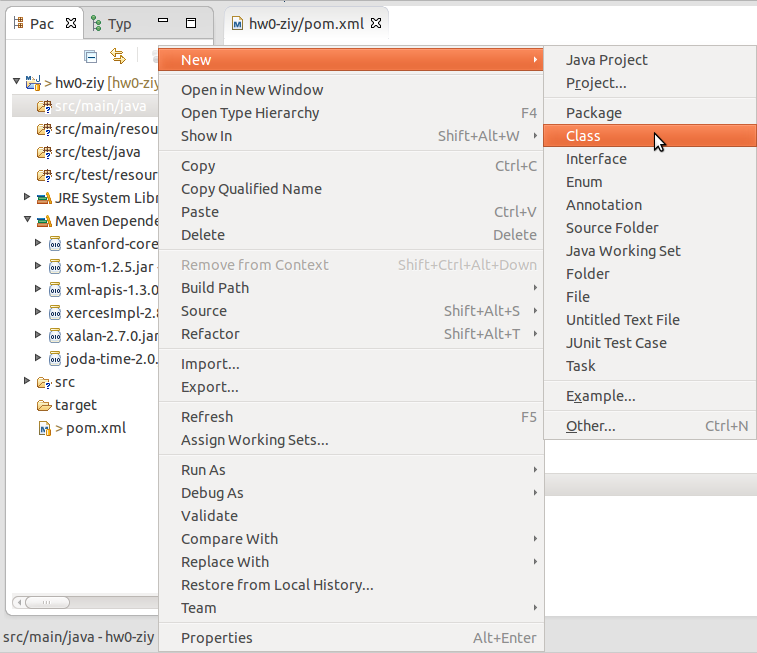
\includegraphics[scale=0.3]{simple-code-01-new-class}
\caption{Creating a new Java class\label{simple-code-01-new-class}}
\end{figure}

\begin{enumerate}

\item Now, you need to create a new Java class by right-clicking
\textbf{src/main/java}, and select \textbf{New} $\rightarrow$ \textbf{Class}.
See Figure \ref{simple-code-01-new-class}.

\begin{figure}
\centering
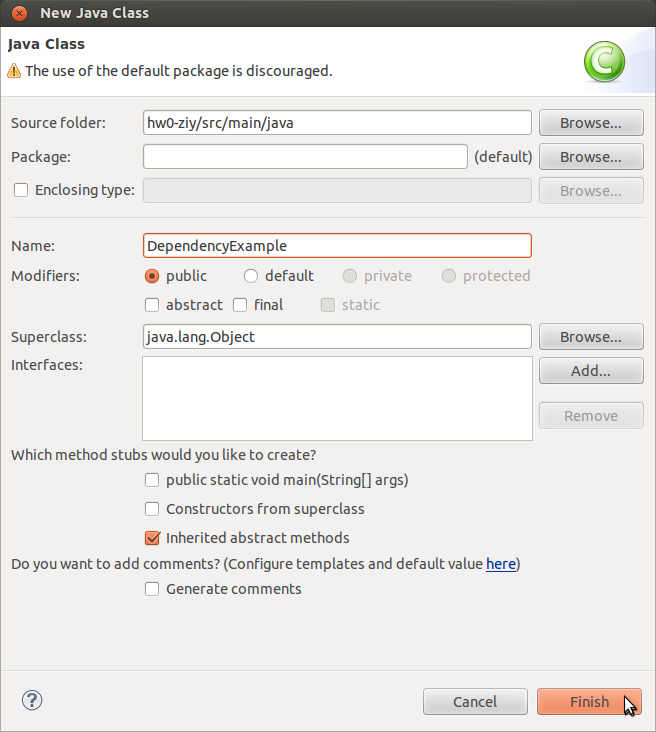
\includegraphics[scale=0.3]{simple-code-02-classname}
\caption{Typing in the classname\label{simple-code-02-classname}}
\end{figure}

\item In the popup window, keep the \textbf{Package} as blank (aka default
package), and type in ``DependencyExample'' next to \textbf{Name}. Please do not
try to specify a different name or package, because our evaluation script will
try to evaluate your submission by looking for the main method within
\texttt{src/main/java/DependencyExample}. Click \textbf{Finish} to proceed.

\lstinputlisting[language=Java,float,linewidth=1.1\textwidth,caption=A simple
tokenization program based on Stanford CoreNLP
tool,label=java]{DependencyExample.java}

\item Now, the Java Editor will be automatically opened to allow you to edit
your Java code. Please copy the content from Listing \ref{java} to your Java
code.

\begin{figure}
\centering
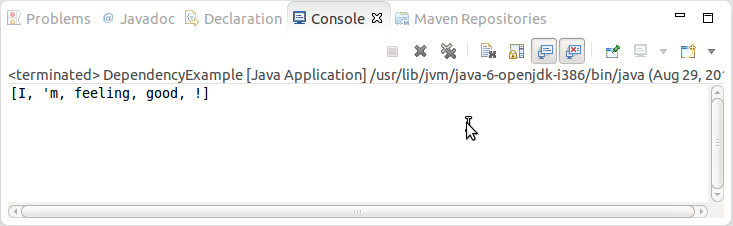
\includegraphics[scale=0.3]{simple-code-04-run}
\caption{Showing tokenization result\label{simple-code-04-run}}
\end{figure}

\item You could try to test your code with some simple sentence, e.g., ``I'm
feeling good!''. Your output should be the same as in Figure
\ref{simple-code-04-run}. That looks good, right? It can split ``'m'' from ``I''
and can keep punctuations (``!'').

\begin{qa}

\item[Q1] How can I run the Java code within Eclipse? And how can I send command
line arguments in Eclipse?

\item[A1] These are Eclipse/Java related questions. You can refer to
\\\url{http://www.javaprogrammingforums.com/java-jdk-ide-tutorials/362-how-send-command-line-arguments-eclipse.html}
or search for other similar posts or articles.

\end{qa}

\end{enumerate}
